\documentclass[letterpaper,12pt,fleqn]{article}
\usepackage{matharticle}
\usepackage{mathtools}
\usepackage{tikz}
\pagestyle{plain}
\begin{document}

\begin{center}
\Large Math-19 Homework \#3 Solutions
\end{center}

\vspace{0.5in}

\underline{Reading}

Please read sections 1.8 through 1.12 and do all concept problems in the posted
sections on web\-assign.

\underline{Problems}

\begin{enumerate}
\item Solve for $x$.  Remember, the answer should be a subset of the real
numbers expressed in interval notation --- not just single numbers.
\[\frac{x^{\frac{5}{2}}-3x^{\frac{3}{2}}-10x^{\frac{1}{2}}}{x^2-9x+20}\ge0\]

\begin{eqnarray*}
\frac{x^{\frac{5}{2}}-3x^{\frac{3}{2}}-10x^{\frac{1}{2}}}{x^2-9x+20} &\ge& 0 \\
\frac{x^{\frac{1}{2}}(x^2-3x-10)}{x^2-9x+20} &\ge& 0 \\
\frac{x^{\frac{1}{2}}(x-5)(x+2)}{(x-5)(x-4)} &\ge& 0 \\
\frac{x^{\frac{1}{2}}(x+2)}{x-4} &\ge& 0\hspace{0.25in}x\ne5 \\
\end{eqnarray*}

So far, we have $x\ne5$. Also, the $x^{\frac{1}{2}}$ factor means $x\ge0$. We need
a sign table to resolve the sign of the remaining terms:

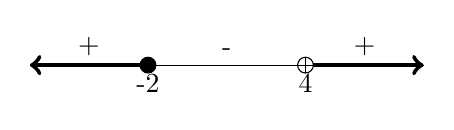
\begin{tikzpicture}
\draw (0,0) -- (5,0);
\draw (1.5,0.1) -- (1.5,-0.1);
\draw (3.5,0.1) -- (3.5,-0.1);
\draw [fill=black] (1.5,0) circle [radius=0.1];
\draw (3.5,0) circle [radius=0.1];
\node [below] at (1.5,0) {-2};
\node [below] at (3.5,0) {4};
\node [above] at (0.75,0) {+};
\node [above] at (2.5,0) {-};
\node [above] at (4.25,0) {+};
\draw [->,ultra thick] (3.6,0) -- (5,0);
\draw [<-,ultra thick] (0,0) -- (1.4,0);
\end{tikzpicture}

\begin{tabular}{|c|c|c|c|}
\hline
$x$ & $x+2$ & $x-4$ & sign \\
\hline
-3 & - & - & + \\
\hline
0 & + & - & - \\
\hline
5 & + & + & + \\
\hline
\end{tabular}

Taking the intersection of all three conditions we get:
$(4,5)\bigcup(5,\infty)$. But note, because of the $\sqrt{x}$ factor, $x=0$
works. So the final answer is: $\{0\}\bigcup(4,5)\bigcup(5,\infty)$.

\bigskip

\item We want a circle whose diameter is the line segment between the points
$(5,4)$ and $(-3,-2)$. Using the distance and midpoint formulas:
\begin{enumerate}
\item{Determine the center of the circle.}

This is the midpoint of the diameter:
\[\left(\frac{5-3}{2},\frac{4-2}{2}\right)=
    \left(\frac{2}{2},\frac{2}{2}\right)=(1,1)\]

\item{Determine the radius of the circle.}

First, determine the length of the diameter:
\begin{eqnarray*}
d &=& \sqrt{(5+3)^2+(4+2)^2} \\
    &=& \sqrt{8^2+6^2} \\
    &=& \sqrt{64+36} \\
    &=& \sqrt{100} \\
    &=& 10 \\
\end{eqnarray*}
The radius is half the diameter, so $r=5$.

\bigskip

\item{What is the equation of the circle in standard form?}
\[(x-1)^2+(y-1)^2=25\]

\item{What is the equation of the circle in general form?}
\begin{eqnarray*}
(x-1)^2+(y-1)^2 &=& 25 \\
(x^2-2x+1)+(y^2-2y+1)-25 &=& 0 \\
x^2-2x+y^2-2y-23 &=& 0 \\
\end{eqnarray*}
\end{enumerate}

\item Find the equation of the line containing the diameter in question (2):
\begin{enumerate}
\item{In point/slope form.}
\[m=\frac{4+2}{5+3}=\frac{6}{8}=\frac{3}{4}\]
\[y-4=\frac{3}{4}(x-5)\]
or
\[y+2=\frac{3}{4}(x+3)\]

\item{In slope-intercept form.}
\[y-4=\frac{3}{4}(x-5)\]
\[y-4=\frac{3}{4}x-\frac{15}{4}\]
\[y=\frac{3}{4}x-\frac{15}{4}+4\]
\[y=\frac{3}{4}x+\frac{1}{4}\]

\item{In general form.}
\[y=\frac{3}{4}x+\frac{1}{4}\]
\[4y=3x+1\]
\[3x-4y+1=0\]

\item{Find the equation of the line through the center of the circle and
perpendicular to the line containing the stated diameter.}
\[\frac{3}{4}m=-1\]
\[m=-\frac{4}{3}\]
\[y-1=-\frac{4}{3}(x-1)\]
\end{enumerate}

\item The amount of heat energy ($Q$) needed to change the temperature of an
object (without going through a phase change like melting or boiling) is jointly
proportional to the mass of the object ($m$) and the \emph{change} in
temperature ($\Delta T$).
\begin{enumerate}
\item Write an equation that models this physical phenomenon. Use $c$ for the
constant of proportionality.
\[Q=cm\Delta T\]

\item The MKS unit for heat energy is the Joule (J). The constant of
proportionality is specific to the substance being heated and is referred to as
the \emph{specific heat} of the substance. If $Q$ is measured in Joules ($J$),
$m$ is measured in grams ($g$), and temperature is measured in Kelvin (K), what
are the units of $c$?
\[Q=cm\Delta T\]
\[J=c(g)(K)\]
\[c=Jg^{-1}K^{-1}\]

\item In the lab, it is found that $41790J$ of heat energy raises the
temperature of $1L$ of water by $10K$. What is the specific heat of water?
(1L of water=1000g)
\begin{eqnarray*}
41790J &=& c(1L)\left(\frac{1000g}{1L}\right)(10K) \\
41790J &=& c(10000gK) \\
c &=& 4.179 Jg^{-1}K^{-1} \\
\end{eqnarray*}
You can actually look this up in any specific heat table on the internet or in
your chemistry book.
\end{enumerate}

\bigskip

\item Consider the equation:
\[y=x^2+2x-5\]
For each of the parts below, use the graphing functions under the \emph{math}
(TI-89) or \emph{calc} (TI-83/84) menus to find the answer and submit a
screen-shot from your calculator that shows the correct answer.
\begin{enumerate}
\item Find the $y$-value when $x=1.3$ using the \emph{value} function.
\item Find the $x$-intercepts using the \emph{zero} function.
\item Determine the minimum value using the \emph{minimum} function.
\item Determine the $x$-values for $y=5$ using the \emph{intersect} function.
Note that you will need to add something to your graph to do this. Also note
that there are multiple answers.
\item Now graph the function $y=x^2+11$. Huh!? Nothing seems to appear! Why,
and how can you fix this? Submit a screen shot that uses your fix.

\bigskip

See hw03-calc.pdf
\end{enumerate}

\end{enumerate}
\end{document}
